\documentclass{article}
\usepackage{tabularx}
\usepackage{longtable}
\usepackage{array}
\usepackage{float}
\usepackage{listings}
\usepackage{amsmath}
\usepackage{amssymb}
\usepackage{mathtools}
\usepackage{amsfonts}
\usepackage{graphicx}
\usepackage[table]{xcolor}
\setlength{\arrayrulewidth}{0.5mm}
\graphicspath{ {./images} }
\usepackage[margin=20mm]{geometry}
\renewcommand{\labelenumii}{\theenumii}
\renewcommand{\theenumii}{\theenumi.\arabic{enumii}.}
\renewcommand{\arraystretch}{1.5}
\newcommand{\f}[2]{f_{#1}(#2)}
\newcommand{\code}[1]{\texttt{#1}}
\DeclarePairedDelimiter{\ceil}{\lceil}{\rceil}
\DeclarePairedDelimiter{\set}{\left\{}{\right\}}
\DeclarePairedDelimiter{\parens}{\lparen}{\rparen}
\title{HW2 Report}
\date{}
\begin{document}
\maketitle
\section*{Q2:}
    \begin{figure}[H]
        \centering
        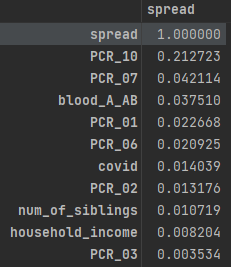
\includegraphics{images/q2.png}
        \caption{The 10 most correlated features to \code{spread}}
    \end{figure}
\section*{Q3:}
    \begin{figure}[H]
        \centering
        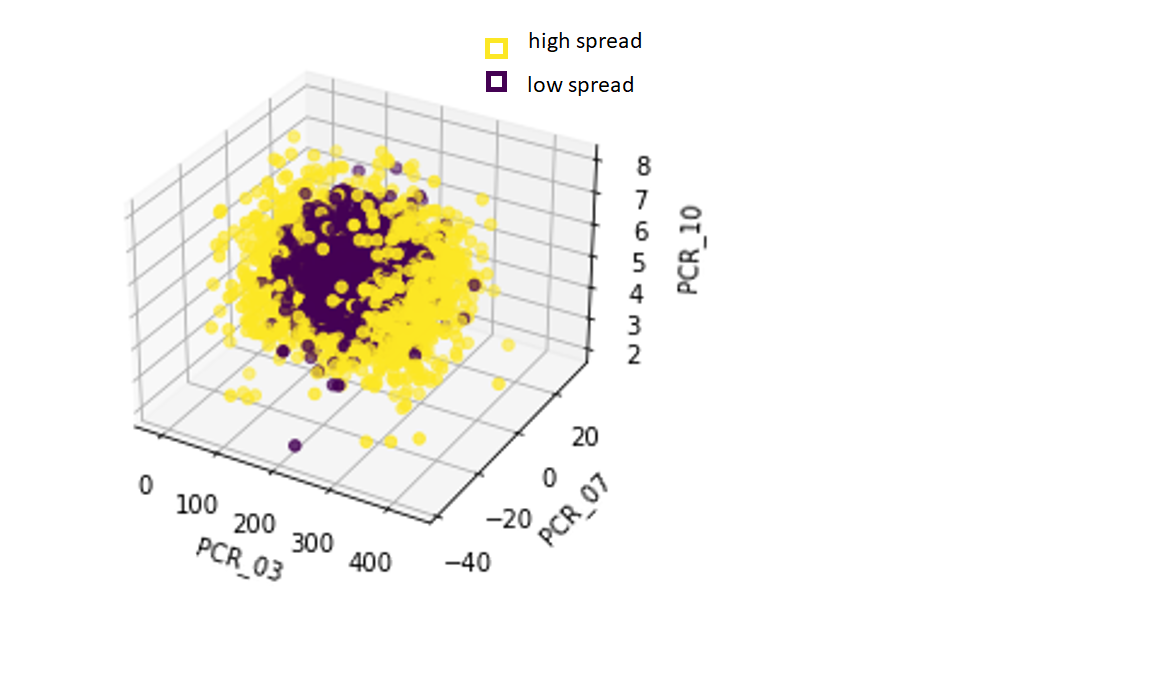
\includegraphics{images/q3.png}
        \caption{3D Scatter plot of \code{PCR\_03}, \code{PCR\_07}, and \code{PCR\_10} according to \code{spread}}
    \end{figure}
\section*{Q4:}
\section*{Q6:}
    \paragraph*{}
    Z-score scaling scales the data of a feature by ensuring that they have zero mean and unit variance. What this means is that features scaled according to this technique have their outliers handled correctly, whereas the scale between different features may vary. This technique would be preferably used on features which already follow a normal or close to normal distribution and or have many significant outliers. On-the-other-hand, the min-max technique involves scaling the data of a feature to a specific range (generally between 0 and 1). Contrary to the Z-score method, this technique guarantees uniform scale across features, but does not handle outliers well. Therefore, it would be preferable to use this technique when the feature in question has no significant outliers and or does not follow a normal distribution.

\end{document}